\documentclass{report}
\usepackage[latin1]{inputenc}
\usepackage{amsmath}
\usepackage{amsfonts}
\usepackage{amssymb}
\usepackage{graphicx}
\usepackage{subeqn}
\usepackage{enumerate}
\setlength{\oddsidemargin}{0pt}
\setlength{\textwidth}{463pt}
\setlength{\marginparsep}{0pt}
\setlength{\marginparwidth}{60pt}
\setlength{\topmargin}{0pt}
\setlength{\headheight}{0pt}
\setlength{\headsep}{0pt}
\setlength{\textheight}{650pt}
\setlength{\footskip}{0pt}
\newtheorem{theorem}{Theorem}[section]
\def\bibname{Referencias}
\def\chaptername{Cap\'{\i}tulo }
\def\contentsname{Contenido}
\def\appendixname{Ap\'endice}
\newtheorem{teorema}[theorem]{Teorema}
\newtheorem{lema}[theorem]{Lema}
\newtheorem{corolario}[theorem]{Corolario}
\newtheorem{proposicion}[theorem]{Proposici\'on}
\newtheorem{observacion}[theorem]{Observaci\'on}
\newtheorem{ejem}[theorem]{Ejemplo}
\newtheorem{ejemplo}[theorem]{Ejemplos}
\newtheorem{nota}[theorem]{Nota}
\newtheorem{notacion}[theorem]{Notaci\'on}
\newtheorem{definicion}[theorem]{Definici\'on}
\newtheorem{obs}[theorem]{Observaciones}
\newtheorem{condiciones}[theorem]{Condiciones}
\newcommand{\demostracion}{{\it \bf Demostraci\'on:  }}
\newcommand{\es}[1]{\hspace{.#1 cm}}
\newcommand{\bge}{\begin{equation}}
\newcommand{\ede}{\end{equation}}
\newcommand{\dlxaster}{\nabla _x {\cal L}(x^*,\lambda^*)}
\newcommand{\dfxaster}{\nabla f(x^*)}
\newcommand{\cl}[1]{{\cal #1}} %capitar leter
%\newcommand{\igu}{c_i(x), i \in \cal E}
%\newcommand{\des}{c_i(x), i \in \cal I}
%\renewcommand{\thenumb}{}
%$\stackrel{\tiny def}{=}$
\setlength{\parskip}{1ex plus 0.5ex minus 0.2ex}



\newcommand{\pphi}{{$\phi: NND(s)\rightarrow \Re$}}
\begin{document}
\chapter{Optimizaci\'on con restricciones}
La  optimizaci\'on con restricciones se refiere a la
minimizaci\'on de funciones sujeta a restricciones sobre las
variables. Una formulaci\'on general de estos problemas es

\begin{equation}
\min_{x \in \Re^n} f(x) \mbox { sujeto a } \left\{
\begin{array}{ll}
c_i(x)=0,& i \in {\cal E} \\
c_i(x) \geq 0, & i  \in {\cal I},
\end{array} \right.
\label{problgeneral}
\end{equation}

\noindent donde las funciones $f$ y $c_i$ son funciones suaves de
valor real definidas  sobre un subconjunto de $\Re^n$, y ${\cal
E}$ e ${\cal I}$ son dos conjuntos finitos de indices. En lo
sucesivo se llamar\'a a $f$ la funci\'on objetivo, mientras que
$c_i$, $i \in {\cal E}$ y $c_i$, $i \in {\cal I}$ son las {\it
restricciones} de {\it igualdad} y de {\it desigualdad}
respectivamente. Se define el conjunto factible $\Omega$ como el
conjunto de puntos que satisfacen las restricciones, esto es,


\begin{equation}
    \Omega = \left \{x \mid c_i(x)=0, \es{1} i \in {\cal E}; \es{2}
    c_i(x) \geq 0, \es{1} i \in {\cal I} \right\},
\label{defomega}
\end{equation}

\noindent as{\'i} se puede reescribir el problema
(~\ref{problgeneral}) de forma m\'as compacta como

\begin{equation}
\min_{x \in \Omega} f(x). \label{12.3}
\end{equation}

\noindent En este cap{\'i}tulo se derivar\'an las condiciones que
caracterizan las soluciones de ({~\ref{12.3}}).

\section{Soluciones locales y globales}

\noindent Las definiciones de los diferentes tipos de soluciones
locales son extensiones sencillas de las definiciones
correspondientes para el caso sin restricciones, excepto que ahora
nos limitamos a considerar puntos factibles en la vecindad de
$x^*$. Se tienen las siguientes definiciones.

\noindent Un vector $x^*$ es una {\it soluci\'on local} del
problema ({~\ref{12.3}}) \es{1} si $x^* \in \Omega$ y existe una
vecindad ${\cal N}$ de $x^*$ tal que $f(x) \geq f(x^*)$ para $x
\in {\cal N} \cap \Omega$.

\noindent Un vector $x^*$ es una {\it soluci\'on local estricta}
(tambi\'en {\it llamada solucion local fuerte}) si $x^* \in
\Omega$ y existe una vecindad ${\cal N}$ de $x^*$ tal que $f(x) >
f(x^*)$ para $x \in {\cal N} \cap \Omega$ con $x \neq x^*$.

%\ejem
\begin{ejem}
\begin{equation} \min x_1+x_2 \es{2} \text{sujeto  a } \es{2}
x_1^2+x_2^2-2=0. \label{12.9}
\end{equation}
\end{ejem}


\begin{figure}
\centering
\includegraphics[width=2.5in]{Fig123.ps}
\caption{Problema (~\ref{12.9}), se muestran los gradientes de las
restricciones y de la funci\'on objetivo en varios puntos
factibles.} \label{Fig123}
\end{figure}

%(ver figura ***).
En este caso se tiene $f(x)=x_1+x_2$, ${\cal I}=\emptyset$, ${\cal
E}=\{1\}$, y $c_1(x)=x_1^2+x_2^2-2$. Por inspecci\'on se puede ver
que el conjunto factible es el circulo de radio $\sqrt{2}$
centrado en el origen (\'unicamente la frontera del circulo no su
interior). No es dif{\'i}cil verificar  que la soluci\'on $x^*$ es
$(-1,-1)^T$. Desde cualquier otro punto sobre el circulo es
sencillo encontrar un camino en el que los puntos que lo formen
sean factibles y al mismo tiempo se este decrementando la funcion
a lo largo de el. Por ejemplo, partiendo del punto
$x=(\sqrt{2},0)^T$ cualquier movimiento en la direcci\'on del
movimiento de las manecillas del reloj alrededor del circulo tiene
el efecto deseado.

De la Figura (~\ref{Fig123}) podemos ver que en la soluci\'on
$x^*$, la {\it restricci\'on normal} $\nabla c_1(x^*)$ es paralela
a $\nabla f(x^*)$. Esto es, existe un escalar $\lambda_1^*$ tal
que

\begin{equation}
\nabla f(x^*)=\lambda_1^*\nabla c_1(x^*). \label{12.10}
\end{equation}

\noindent (En este caso se tiene $\lambda_1^*=-\frac{1}{2}$.)
\vspace{1cm}

Se puede encontrar anal{\'i}ticamente (~\ref{12.10}) al aproximar
la funci\'on objetivo y  las restricciones con su serie de Taylor
de primer orden correspondiente. Para mantener la factibilidad con
respecto a la funcion  $c_1(x)=0$, se requiere que $c_1(x+d)=0$;
esto es,

\begin{equation}
0 = c_1(x+d)\approx c_1(x)+\nabla c_1(x)^Td=\nabla c_1(x)^Td.
\label{12.11}
\end{equation}

\noindent De donde, la direcci\'on $d$ se mantiene factible con
respecto a $c_1$, cuando esta satisface

\begin{equation}
\nabla c_1(x)^Td=0. \label{12.12}
\end{equation}

\noindent De forma similar, una direcci\'on de mejora debe generar
un decremento en $f$, as{\'i} que

\begin{center}
$$0>f(x+d)-f(x)\approx \nabla f(x)^Td,$$
\end{center}

\noindent o bien,

\begin{equation}
\nabla f(x)^Td<0. \label{12.13}
\end{equation}

\noindent Si existe una direcci\'on $d$ que satisface
(~\ref{12.12}) y (~\ref{12.13}) entonces se concluye que es
posible tener una mejora en el punto actual $x$. De aqui se sigue
que una condici\'on {\it necesaria} de optimalidad para el
problema (~\ref{12.9}) es que no exista una direcci\'on $d$ que
satisfaga tanto (~\ref{12.12}) como (~\ref{12.13}).

Por medio de un dibujo, el lector puede verificar que la \'unica
forma en que dicha direcci\'on no exista es que $\nabla f(x)$ y
$\nabla c_1(x)$ sean paralelos, esto es, $\nabla f(x)=\lambda_1
\nabla c_1(x) $ para alg\'un escalar $\lambda_1$. En caso de que
esta condici\'on no se satisfaga, la direcci\'on definida por


\begin{equation}
d = -\left(I-\frac{\nabla c_1(x) \nabla c_1(x)^T}{\|\nabla
c_1(x)\|^2} \right ) \nabla f(x)
 \label{12.14}
\end{equation}

\noindent satisface las condiciones (~\ref{12.12}) y
(~\ref{12.13}).

Ahora se introduce la {\it funci\'on Lagrangiana}

\begin{equation}
{\cal L} (x,\lambda_1)=f(x)-\lambda_1c_1(x), \label{12.15}
\end{equation}

\noindent y observe que $\nabla_x {\cal L}(x,\lambda_1)=\nabla
f(x)-\lambda_1 \nabla c_1(x)$ de modo que se puede reescribir la
condici\'on (~\ref{12.10}) como: en la soluci\'on $x^*$, existe un
escalar $\lambda_1^*$ tal que

\begin{equation}
\nabla_x {\cal L}(x^*,\lambda_1^*)=0. \label{12.16}
\end{equation}

Esto \'ultimo sugiere que la soluci\'on del problema con
restricciones de igualdad se calcula encontrando los puntos
estacionarios de la funci\'on de Lagrange. El escalar $\lambda_1$
es llamado el {\it multiplicador de Lagrange} para la
restricci\'on $c_1(x)=0$.

Observar que  la condici\'on (~\ref{12.10}) (equivalentemente
~\ref{12.16}) parece ser una condici\'on {\it necesaria} para una
soluci\'on \'optima  de el problema (~\ref{12.9}), pero no es {\it
suficiente}. Por ejemplo en el problema (~\ref{12.9}),
(~\ref{12.10}) se satisface en el punto $x=(1,1)$ (con
$\lambda=\frac{1}{2}$) pero este punto no es una soluci\'on (de
hecho este punto maximiza la funci\'on objetivo en el circulo).
M\'as a\'un, en el caso de problemas con restricciones de
igualdad, la condici\'on (~\ref{12.10}) no puede considerarse
suficiente simplemente colocando alguna restricci\'on sobre el
signo de $\lambda_1$. Para hacer m\'as claro este comentario,
considere reemplazar la restricci\'on $x_1^2+x_2^2-2=0$ por su
negativo $2-x_1^2-x_2^2=0$ en el ejemplo (~\ref{12.9}). La
soluci\'on del problema no se ve afectada pero el valor de
$\lambda_1^*$ que satisface la condicio\'on (~\ref{12.10}) cambia
de $\lambda_1^*=-\frac{1}{2}$ a $\lambda_1^*=\frac{1}{2}$.


Ahora considerese el ejemplo anterior pero con una peque\~na
modificaci\'on, se reemplaza la restricci\'on de igualdad por una
de desigualdad como sigue

\begin{ejem} \label{Ejem.12.2}
\begin{equation} \min x_1+x_2 \es{2} \text{sujeto  a } \es{2}
x_1^2+x_2^2-2 \geq 0. \label{12.17}
\end{equation}
\end{ejem}

En este caso la regi\'on factible es el ciruclo del problema
(~\ref{12.9}) y su interior. Por inspecci\'on se observa que la
soluci\'on sigue siento $(-1,-1)$  y que la condici\'on
(~\ref{12.10}) se cumple para $\lambda_1^*=\frac{1}{2}$.
Sin embargo se tiene que el multiplicador de Lagrange tiene el
signo diferente al encontrado en el ejemplo anterior.

Como antes la conjetura es que un punto $x$ no es optimo si es
posible encontrar un paso $d$ que manteniendo la factibilidad
decremente la funci\'on objetivo $f$ considerando la
aproximaci\'on de primer orden de la funci\'on. Entonces la
direcci\'on $d$ decrementa el valor de la funci\'on objetivo si
$\nabla f(x)^Td<0$, mientras que mantiene la  factibilidad si

\begin{center}
$$0\leq c_1(x+d)\approx c_1(x)+\nabla c_1(x)^Td,$$
\end{center}

\noindent es decir,

\begin{equation}
c_1(x)+\nabla c_1(x)^Td \geq 0. \label{12.18}
\end{equation}

\noindent Para determinar cuando existe una direcci\'on que
satisfaga (~\ref{12.13}) y (~\ref{12.18}) se consideran dos casos.

\noindent{\bf Caso I:} Considerar que $x$ esta estrictamente
dentro del circulo, de modo que la desigualdad estricta $c_1(x)> 0
$ se satisface. En este caso cualquier vector $d$ cumple
(~\ref{12.18}), teniendo cuidado que su longitud sea
suficientement peque\~na. En particular, siempre que $\nabla
f(x^*) \neq 0$, se puede obtener una direcci\'on $d$ que satisgace
(~\ref{12.13}) y (~\ref{12.18}) al tomar

\begin{center}
$$ d = -c_1(x)\frac{\nabla f(x)}{\|\nabla f(x) \|}.$$
\end{center}

\noindent La \'unica situaci\'on en la que esta direcci\'on no
existe es cuando

\begin{equation}
\nabla f(x)=0. \label{12.19}
\end{equation}

\noindent{\bf Caso II:} Ahora consid\'erese el caso en que $x$
esta en la frontera del circulo, de modo que $c_1(x)=0$. Las
condiciones (~\ref{12.13}) y (~\ref{12.18}) son entonces

\begin{equation}
\nabla f(x)d \leq 0, \es{2} \nabla c_1(x)^Td \geq 0. \label{12.19}
\end{equation}

\begin{figure}[h]
\centering
\includegraphics[width=2.5in]{Fig125.ps}
\caption{Una direcci\'on $d$ que satisface (~\ref{12.13}) y
(~\ref{12.18}) que vive en la intersecci\'on de un medio plano
cerrado y un medio plano abierto.} \label{Fig125}
\end{figure}

La primera condici\'on define un espacio  abierto mientras que la
segunda define un espacio cerrado (ver Figura ~\ref{Fig125}). De
la figura es claro que las dos regiones no se intersectan
unicamente cuando $\nabla f(x)$ y $\nabla c_1(x)$ apuntan en la
misma direcci\'on, esto es, cuando

\begin{equation}
\nabla f(x)=\lambda_1 \nabla c_1(x), \es{2} \text{para alg\'un}
\es{1} \lambda_1 \geq 0. \label{12.20}
\end{equation}

Observar que el signo del multiplicador es relevante. Si
(~\ref{12.10}) hubiera sido satisfecha con un valor {\it negativo}
de $\lambda_1$, entonces $\nabla f(x)$ y $\nabla c_1(x)$
apuntar{\'i}an en direcci\'on opuesta y entonces las direcciones
que satisfacen (~\ref{12.13}) y (~\ref{12.18}) formar{\'i}an un
medio plano abierto.

Las condicione \'optimas en ambos casos pueden ser resumidas como
sigue. Cuando no existen direcciones factibles de descenso de
primer orden en alg\'un punto $x^*$, se tiene que

\begin{equation}
\nabla_x {\cal L}(x^*,\lambda_1^*)=0, \es{2} \text{para alg\'un}
\es{1} \lambda_1^* \geq 0, \label{12.21}
\end{equation}

\noindent donde tambi\'en se requiere que

\begin{equation}
\lambda_1^* c_1(x^*)=0. \label{12.22}
\end{equation}

Esta condici\'on es conocida como la {\it condici\'on de
complementariedad}, \'esta implica que el multiplicador de
Lagrange $\lambda_1$ puede ser estrictamente positivo {\it
\'unicamente cuando la restricci\'on correspondiente $c_1$ esta
activa}. En el caso I, se ten{\'i}a que $c_1(x^*)>0$, as{\'i} que
(~\ref{12.22}) requiere que $\lambda_1^*=0$. Luego, (~\ref{12.21})
se reduce a $\nabla f(x^*)=0$, como se necesitaba en
(~\ref{12.19}). En el caso II, (~\ref{12.22}) permite a
$\lambda_1^*$ tomar valores no negativos, as{\'i} (~\ref{12.21})
resulta ser equivalente a (~\ref{12.20}).

\noindent Ahora se agrega una restricci\'on al problema
~\ref{12.17}

\begin{ejem} \label{Ejem.12.3}
\begin{equation} \min x_1+x_2 \es{2} \text{sujeto  a } \es{2}
x_1^2+x_2^2-2 \geq 0, x_2 \geq 0, \label{12.23}
\end{equation}
\end{ejem}

\noindent para el cual la regi\'on factible es la mitad del disco
que se muestra en el (Figura ~\ref{Fig126}). No es dif{\'i}cil ver
que la soluci\'on es $(-\sqrt{2},0)^T$, un punto en el que ambas
restricciones estan activas. Al repetir los argumentos que se
utilizaron en los ejemplos anteriores, se concluye que una
direcci\'on  $d$ es una direcci\'on de descenso factible de primer
orden, si satisface las siguientes condiciones:

\begin{figure}
\centering
\includegraphics[width=2.5in]{Fig126.ps}
\caption{Una direcci\'on $d$ que satisface (~\ref{12.13}) y
(~\ref{12.18}) que vive en la intersecci\'on de un medio plano
cerrado y un medio plano abierto.} \label{Fig126}
\end{figure}

\begin{equation}
\nabla c_i(x)^T \geq 0, \es{2} i \in {\cal I}={1,2}, \es{2} \nabla
f(x)^Td<0. \label{12.24}
\end{equation}

Sin embargo es claro de la (Figura ~\ref{Fig126}) que esta
direcci\'on no puede existir cuando $x = (-\sqrt{2},0)^T$. Las
condiciones $\nabla c_i(x)^T \geq 0, \es{1} i=1,2$ son satisfechas
ambas solo si $d$ esta en el cuadrante definido por $\nabla
c_1(x)$ y $\nabla c_2(x)$, pero por inspecci\'on es claro que
todos los vectores $d$ en este cuadrante satisfacen $\nabla
f(x)^Td \geq 0$.

Ahora se revisa el comportamiento de el Lagrangiano y sus
derivadas en el problema (~\ref{12.23}) y el punto soluci\'on
$(-\sqrt{2},0)^T$. Primero se incluye un t\'ermino adicional
$\lambda_1c_i(x)$ en el Lagrangiano para cada restricci\'on
adicional, de modo que se tiene

%\begin{center}
$${\cal L}(x,\lambda)=f(x)-\lambda_1 c_1(x) -\lambda_2 c_2(x),$$
%\end{center}

\noindent donde $\lambda=(\lambda_1,\lambda_2)^T$ es el vector de
multiplicadores de Lagrange. La extensi\'on de la condicio\'on
(~\ref{12.21}) en este caso es

\begin{equation}
\nabla_x {\cal L}(x^*, \lambda^*)=0, \es{2} \text {para alg\'un}
\es{1} \lambda^* \geq 0, \label{12.25}
\end{equation}


\noindent donde la desigualdad $\lambda^* \geq 0$ significa que
todos los componentes de $\lambda^*$ son no negativos. Al aplicar
las condiciones de complementariedad (~\ref{12.22}) a ambas
restricciones de desigualdad, se obtiene

\begin{equation}
\lambda_1^*c_1^*(x)=0, \es{2} \lambda_2^*c_2^*(x)=0. \label{12.26}
\end{equation}

\noindent Cuando $x^*=(-\sqrt{2},0)^T$, tenemos

\bge  \nabla f(x^*) = \left [
\begin{array}{c}
$$1$$ \\
$$1$$
\end{array}
\right ], \es{3} \nabla c_1(x^*) = \left [
\begin{array}{c}
$$2\sqrt{2}$$\\
$$0$$
\end{array}
\right ], \es{3} \nabla c_2(x^*) = \left [
\begin{array}{c}
$$0$$\\
$$1$$
\end{array}
\right ], \ede


\noindent as{\'i} que es sencillo verificar que $\nabla_x {\cal
L}(x^*,\lambda^*)=0$ cuando se selecciona $\lambda^*$ como sigue:

\begin{equation}
\lambda^* =  \left [
\begin{array}{c}
1/(2\sqrt{2})\\
1
\end{array} \right ].
\end{equation}

\noindent Observar que las componentes de $\lambda^*$ son
positivas.

Ahora se consideran algunos otros puntos factibles que no son
soluci\'on de (~\ref{12.23}) y se examinan las propiedades de el
Lagrangiano y su gradiente en estos puntos.

Para el punto $x=(\sqrt{2}, 0)^T$ se tiene que ambas restricciones
estan activas. Sin embargo el gradiente de la funci\'on objetivo
$\nabla f(x)$ ya no vive en el cuadrante definido por las
condiciones $\nabla c_i(x)^Td\geq 0$, $i=1,2$. Una direcci\'on de
descenso factible de primer orden de este punto (un vector que
satisface (~\ref{12.24})) es simplemente $d=(-1,0)^T$; hay muchos
otros. Para este valor de $x$ es sencillo verificar que la
condici\'on $\nabla _x \cl{L}(x,\lambda)=0$ se satisface
\'unicamente cuando $\lambda=(-1/(2\sqrt{2}),1)$. Observar que la
primera componente  $\lambda_1$ es negativa, as{\'i} que las
condiciones (~\ref{12.25}) no se cumplen en este punto.

Finalmente, consideremos el punto $x=(1,0)^T$, en el cual solo la
segunda restricci\'on $c_2$ esta activa. En este punto,
linealizaciones de $f$ y de $c$ como en el Ejemplo
~\ref{Ejem.12.2} dan las siguientes condiciones, las cuales deben
 cumplirse para que  $d$ sea una direcci\'on de descenso
factible, de primer orden:

\bge \label{12.27} 1 + \nabla c_1(x)^Td\geq 0, \es{3} \nabla
c_2(x)^T d \geq 0, \es{3} \nabla f(x)^Td<0. \ede

De hecho solo se debe verificar que se satisfagan la segunda y
tercera condici\'on ya que siempre se satisface la primera al
multiplicar $d$ por una cantidad positiva lo suficientemente
peque\~na. Observar que

\bge  \nabla f(x) = \left [
\begin{array}{c}
$$1$$ \\
$$1$$
\end{array}
\right ], \es{3} \nabla c_2(x) = \left [
\begin{array}{c}
$$0$$\\
$$1$$
\end{array}
\right ], \ede


\noindent es sencillo verificar que el vector
$d=-(\frac{1}{2},\frac{1}{4})$ satisface (~\ref{12.27}) y que es
por lo tanto una direcci\'on de descenso.

Para mostrar que las condiciones de optimalidad (~\ref{12.25}) y
(~\ref{12.26}) fallan, se observar de (~\ref{12.26}) que debido a
que $c_1(x)>0$, se debe cumplir que $\lambda_1=0$. Por lo tanto,
al tratar de satisfacer $\nabla _x \cl{L}(x,\lambda)=0$, se esta
buscando un valor $\lambda_2$ tal que $\nabla f(x)-\lambda_2
\nabla c_2(x)=0$. Ya que $\lambda_2$ con esta caracter{\'i}stica
no existe, este punto no satisface las condiciones de optimalidad.


\section{Condiciones de optimalidad de primer orden}

{\large {\bf Establecimiento de las condiciones necesarias de
primer orden}}

Ahora se generalizan las observaciones hechas en los ejemplos
anteriores.

En general, el Lagrangiano para el problema de optimizaci\'on con
restricciones (~\ref{problgeneral}) se define como


\bge \label{12.28}
{\cal L}(x,\lambda)=f(x)- \sum_{i \in {\cal E}
\cup {\cal I}} \lambda_i c_i(x).
\ede

El {\it conjunto activo} ${\cal A}(x)$ para cualquier punto
factible $x$ es la uni\'on del conjunto ${\cal E}$ con los indices
de las restricciones de desigualdad activas, esto es,

\bge \label{12.29} {\cal A}(x)= {\cal E} \cup \{i \in {\cal I}\mid
c_i(x)=0\}. \ede

Es importante considerar que es posible que $\nabla c_i(X)$ se
anule debido a la representaci\'on algebraica de $c_i$, de modo
que el t\'ermino $\lambda_i \nabla c_i(x)$ se anula para todos los
valores de $\lambda_i$. Lo que usualmente se hace para evitar este
comportamiento degenerado en el valor de $x$ en cuestion es
establecer un supuesto sobre las restricciones como sigue.

\begin{definicion} (LICQ).
Dado el punto $x^*$ y el conjunto activo ${\cal A}(x)$ definido
por (~\ref{12.29}) se dice que se satisface la condici\'on de
independencia lineal en las restricciones (por sus siglas en
ingl\'es LICQ) si el conjunto de gradientes de las restricciones
activas ${\nabla c_i(x^*), i \in {\cal A}(x^*) }$ es linealmente
independiente.
\end{definicion}


Esta condici\'on permite establecer las condiciones de optimalidad
para el problema general de optimizaci\'on con restricciones
(~\ref{problgeneral}).

\begin{theorem} \label{Teo12.1} (Condiciones de optimalidad de primer orden)
Sea $x^*$ una soluci\'on local del problema (~\ref{problgeneral})
en donde la condici\'on {\it LICQ} se satisface, entonces hay un
vector multiplicador de Lagrange $\lambda^*$, con componentes
$\lambda^*_i, i \in {\cal E} \cup {\cal I}$, tal que las
siguientes condiciones se satisfacen en $(x^*, \lambda^*)$

\begin{subequations} \label{12.30}

\bge \label{12.30a} \nabla _x {\cal L}(x^*, \lambda^*)=0, \ede

\bge \label{12.30b} c_i(x^*)=0, \es{2} \text{para toda} \es{2} i
\in {\cal E}, \ede

\bge \label{12.30c} c_i(x^*) \geq 0, \es{2} \text{para toda}
\es{2} i \in {\cal I}, \ede

\bge \label{12.30d} \lambda^*_i \geq 0, \es{2} \text{para toda}
\es{2} i \in {\cal I}, \ede

\bge \label{12.30e} \lambda^*_i c_i(x^*)=0,  \es{2} \text{para
toda} \es{2} i \in {\cal E} \cup {\cal I}. \ede
\end{subequations}
\end{theorem}



Las condiciones (~\ref{12.30}) son conocidas como las condiciones
de {\it Karush-Kuhn-Tucker } o de forma m\'as breve como las
condiciones {\it KKT}. Debido a que la condici\'on de
complementariedad implica que los multiplicadores de Lagrange
correspondientes a las restricciones de desigualdad son cero, es
posible omitir los terminos de indices $i \notin {\cal A}(x^*)$ en
(~\ref{12.30a}) y reescribir la condici\'on como

\bge \label{12.31} 0=\dlxaster= \dfxaster - \sum_{i \in {\cal
A}(x^*)} \lambda^*_i \nabla c_i(x^*) \ede

\begin{definicion}\label{Def12.2}(Complementariedad estricta)
Dada una soluci\'on local $x^*$ de (~\ref{problgeneral}) y un vector
$\lambda^*$ que satisface (~\ref{12.30}), se dice que la
condici\'on de complementariedad estricta se satisface siempre que
solo uno de los siguientes t\'erminos se anula, $\lambda^*_i$ y
$c_i(x^*)$ para cada {\'i}ndice $i \in {\cal I}$. En otras
palabras, $\lambda^*_i>0$ para toda $i \in \cl{I}\cup
\cl{A}(x^*)$.
\end{definicion}

Para un problema (~\ref{problgeneral})  y una soluci\'on $x^*$
dados, existen muchos vectores $\lambda^*$ para los que las
condiciones (~\ref{12.30}) se cumplen. Sinembargo cuando la
condici\'on LICQ se satisface el \'optimo $\lambda^*$ es \'unico.

\vspace{1cm}

\noindent{\large {\bf Anal{\'i}sis de sensibilidad}}
\vspace{0.5cm}

El valor de cada multiplicador de Lagrange  $\lambda^*_i$ nos dice
algo sobre la {\it sensibilidad} del valor de la funci\'on
objetivo $f(x^*)$ a la presencia de la restricci\'on $c_i$.

Consid\'erese una restricci\'on $i$ activa, y perturbese el lado
derecho de esta restricci\'on un poco, digamos $c_i(x)\geq
-\epsilon \| \nabla c_i(x^*)\|$ en lugar de $c_i(x)\geq 0$.
Suponer que $\epsilon$ es lo suficientemente peque\~na de modo que
la soluci\'on perturbada $x^*(\epsilon)$ contin\'ua teniendo el
mismo conjunto de  restricciones activas y que los multiplicadores
de Lagrange no fueron afectados demasiado con la pertubaci\'on. Se
tiene entonces que

\begin{center}
\begin{eqnarray}\nonumber
-\epsilon \|\nabla c_i(x^*) \| & = &
c_i(x^*(\epsilon))-c_i(x^*)\approx (x^*(\epsilon)-x^*)^T \nabla
c_i(x^*),\\
0 & = & c_j(x^*(\epsilon))-c_j(x^*)\approx (x^*(\epsilon)-x^*)^T
\nabla
c_j(x^*),\\
&&\hspace{6cm} \text{para toda} \es{2} j \in \cl{A}(x^*) \text{ 
con } j\neq i
\end{eqnarray}
\end{center}

\noindent El valor de $f(x^*(\epsilon))$, puede ser estimado con
ayuda de (~\ref{12.30a}). Se tiene


\begin{center}
\begin{eqnarray}\nonumber
f(x^*(\epsilon))-f(x^*) & \approx & (x^*(\epsilon)-x^*)^T\nabla f(x^*)\\
 & = & \sum_{j \in \cl{A}(x^*)}\lambda_j^*(x^*(\epsilon)-x^*)^T
 \nabla c_j(x^*) \\
 & \approx & - \epsilon \|\nabla c_i(x^*)\|\lambda_i^*.
\end{eqnarray}
\end{center}

\noindent Al tomar el l{\'i}mite se tiene que la familia de
soluciones $x^*(\epsilon)$ satisface

\bge \label{12.33}
\frac{df(x^*(\epsilon))}{d\epsilon}=-\lambda_i^* \|\nabla c_i(x^*)
\|. \ede

Un an\'alisis de sensibilidad de este problema podr{\'i}a concluir
que si $\lambda_i^* \|\nabla c_i(x^*)\|$ es grande, entonces el
valor \'optimo es sensible a la existencia de la i-\'esima
restricci\'on, mientras que si es pequen\~o la dependencia no es
tan fuerte. Si $\lambda_i^*$ es exactamente cero para alguna
restricci\'on activa una pequen\~a perturbaci\'on a $c_i$ en
algunas direcciones dificilmente afectar\'a el valor de la
funci\'on objetivo.

\noindent Es importante hacer notar que el an\'alisis anterior
vale a\'un cuando las restricciones sean escaladas.

\section{Derivaci\'on de las condiciones de primer orden}

{\large {\bf Sucesiones factibles}} \vspace{0.5cm}

Dado un punto factible $x^*$, una sucesi\'on
$\{z_k\}^{\infty}_{k=0}$ con $z_k \in \Re^n$ es una {\it
sucesi\'on factible} si se satisfacen las siguientes propiedades:

\begin{enumerate}[i.]
\item $z_k \neq x^*$ para toda $k$;
%\item \begin{array}{cc} lim & z_k = x^*$ \\
%       k \rightarrow \infty & \\
%       \end{array}
\item $lim_{k \rightarrow \infty} z_k = x^*$;
\item $z_k$ es factible para todo valor suficientemente grande de $k$.
\end{enumerate}


\noindent Se define el conjunto de todas las sucesiones factibles
que se acercan a $x$ por $\cl{T}(x)$.

Se caracteriza una soluci\'on local de (~\ref{problgeneral}) como un
punto $x$ en el cual todas las sucesiones factibles  tienen la
propiedad de que $f(z_k) \geq f(x)$ para toda $k$ suficientemente
grande. En lo que sigue se derivan condiciones que se pueden
verificar bajo las cuales esta propiedad se cumple.

Las {\it direcciones l{\'i}mite} de una sucesi\'on factible son
vectores $d$ tales que


\begin{equation}
\lim_{z_k \in S_d} \frac{z_k-x}{\|z_k-x\|} \rightarrow d,
\end{equation}

\noindent donde $S_d$ es alguna subsucesi\'on de
$\{z_k\}_{k=0}^\infty$. En general, una sucesi\'on factible tiene
almenos una direcci\'on factible y muchas tienen m\'as de una.

\vspace{1cm}
%---------------------------------------------
%\hline \vspace{1cm}

\noindent Dado un punto $x$, si es posible elegir una sucesi\'on
factible de $\cl{T}(x)$ tal que la aproximaci\'on de primer orden
de la funci\'on objetivo se incremente mon\'otonamente a lo largo
de la sucesi\'on , entonces $x$ no puede ser un punto \'optimo.

\begin{theorem}\label{Teo.12.2} Sea $x^*$ una soluci\'on local de
(~\ref{problgeneral}), entonces todas las sucesiones factibles
$\{z_k\}$ en $\cl{T}(x^*)$ deben satisfacer

\bge \label{12.37} \nabla f(x^*)^T d \geq 0,
\ede

\noindent donde $d$ es alguna direcci\'on l{\'i}mite de la sucesi\'on
factible.

\end{theorem}


\vspace{1cm} \noindent{\large {\bf Caracterizando las direcciones
l{\'i}mite}} \vspace{0.5cm}
%{\bf Caracterizando las direcciones l{\'i}mite}

El Teorema ~\ref{Teo.12.2} es muy general sin embargo no es
sencillo utilizarlo pues al parecer se hace necesario conocer
todas las direcciones l{\'i}mite  de todas las sucesiones
factibles en $\cl{T}(x)$. En esta secci\'on se muestra que ciertas
cualidades en las restricciones permitir\'an caracterizar las
propiedades  m\'as importantes de $\cl{T}(x)$, y por lo tanto se
podr\'a verificar la condici\'on (~\ref{12.37}) de modo m\'as
sencillo.

En los resultados siguientes  se introduce la notaci\'on $A$ para
representar la matriz cuyas filas son los gradientes de las
restricciones activas en el punto \'optimo, esto es,

\bge \label{12.38} \nabla c_i^* = \nabla c_i(x^*), \es{3}
A^T=[\nabla c_i^*]_{i \in \cl{A}(x^*)}, \es{3} \nabla f^* = \nabla
f(x^*), \ede

\begin{lema}\label{Lem.12.3}
Las siguientes dos afirmaciones son verdaderas
\begin{enumerate}[i.]
\item Siempre que $d \in \Re^n$ sea una direcci\'on l{\'i}mite
de una sucesi\'on factible, entonces \bge \label{12.39} d^T \nabla
c_i^*=0, \es{2} \text{para toda} \es{2} i \in \cl{E}, \es{2} d^T
\nabla c^*_i \geq 0, \es{2} \text{para toda} \es{2} i \in
\cl{A}(x^*) \cap \cl{I}. \ede

\item Si (~\ref{12.39}) se cumple con $\|d \|=1$ y la condici\'on
LICQ se satisface tambi\'en, entonces $d \in \Re^n$ es una
direcci\'on l{\'i}mite de alguna sucesi\'on factible.
\end{enumerate}
\end{lema}

El conjunto de direcciones definido por (~\ref{12.39}) tiene un
papel importante en las condiciones de optimalidad, as{\'i} que
para referencias futuras se le da un nombre al conjunto y se
define formalmente.

\begin{definicion} \label{Def.12.4}

Dado un punto $x^*$ y el conjunto de restricciones activas
$\cl{A}(x^*)$ definido por (~\ref{12.29}), el conjunto $F_1$ se
define como

\bge F_1 = \left \{  \alpha d | \alpha >0,
\begin{array}{ll}
$$d^T \nabla c_i^*=0$$, & \text{para toda} \es{2}  $$i \in {\cal E}$$ \\
%$$d^T \nabla c_i^*\geq 0$$, & \text{para toda} \ed{2} $$i  \in \cl{A}(x^*) \cap {\cal I}$$,
$$d^T \nabla c_i^*\geq 0$$, & \text{para toda} \es{2} $$i  \in \cl{A}(x^*) \cap {\cal I}$$,
\end{array}
\right \} \ede
\end{definicion}

\noindent Observar que $F_1$ es un cono. De hecho, cuando una
restricci\'on es satisfecha, $F_1$ es el cono tangente al conjunto
factible en $x^*$.

\vspace{0.3cm}
\noindent {\large{\bf Introducci\'on a  los multiplicadores de Lagrange}}

El Lema (~\ref{Lem.12.3}) asegura que cuando la condici\'on LICQ
se cumple, el cono $F_1$ es simplemente el conjunto de todos los
multiplos positivos de todas las direcciones l{\'i}mite de todas las
sucesiones facibles posibles. Por lo tanto la condici\'on
(~\ref{12.37}) del Teorema ~\ref{Teo.12.2} se cumple si $\nabla
f(x^*)^T d <0$ para toda $d \in F_1$. Esta condici\'on tambi\'en
parece imposible de verificar  ya que el conjunto $F_1$ tiene una
infinidad de vectores. El siguiente lema brinda una
alternativa.

\begin{lema} \label{Lem.12.4}
No existe direcci\'on $d \in F_1$ para la cual $d^T \nabla f^*<0$
si y solo si existe un vector $\lambda \in \Re^m$ con

\bge \label{12.46} \nabla f^* = \sum_{i \in \cl{A}(x)} \lambda _i
\nabla c_i^* = A(x^*)^T \lambda, \es{3} \lambda _i \geq 0 \es{2}
\text{para} \es{2} i \in \cl{A}(x^*) \cap \cl{I}. \ede
\end{lema}

\vspace{1cm} \noindent{\large{\bf Prueba del Teorema
~\ref{Teo12.1}}} \vspace{0.5cm}

Los lemas (~\ref{Lem.12.3}) y (~\ref{Lem.12.4}) pueden combinarse
para generar las condiciones $KKT$ descritas en el Teorema
~\ref{Teo12.1}. Suponer que $x \in \Re^n$ es un punto factible en
el cual  satisface la condici\'on LICQ. El teorema asegura que
si $x^*$ es una soluci\'on local de (~\ref{problgeneral}),
entonces existe un vector $\lambda^* \in \Re^m$ que satisface las
condiciones (~\ref{12.30}).

En principio se muestra que hay multiplicadores $\lambda_i, i \in
\cl{A}(x^*) $, tales que  (~\ref{12.46}) se satisface. El Teorema
~\ref{Teo.12.2} dice que $d^T \nabla f^* \geq 0$ para todos los
vectores $d$ tales que son direcciones l{\'i}mite de sucesiones
factibles. A partir del Lema ~\ref{Lem.12.3} se sabe que cuando
las condiciones LICQ se cumplen, el conjunto de todas las
direcciones limite posibles es exactamente el conjunto de vectores
que satisfacen las condiciones )~\ref{12.39}). Al colocar estas dos
afirmaciones juntas, se encuentra que todas las direcciones $d$
que satisfacen (~\ref{12.39}) tambi\'en deben cumplir $d^T \nabla
f^* \geq 0$.  Luego,  del Lema ~\ref{Lem.12.4}, se tiene que hay
un vector $\lambda$ para el cual (~\ref{12.46}) se vale, como se
asegur\'o.

Ahora se define el vector $\lambda^*$ como

\bge  \label{12.51} \lambda_i^* = \left \{
\begin{array}{ll}
$$\lambda_i$$, & $$i \in \cl{A}(x^*)$$ \\
$$0$$, & \text{en otro caso}
\end{array}
\right. \ede

\noindent y se muestra que esta elecci\'on de $\lambda^*$, junto
con la soluci\'on local $x^*$, satisface las condiciones
(~\ref{12.30}). Se verifican estas condiciones una a una.

\begin{itemize}
\item La condici\'on (~\ref{12.30a}) se sigue inmediatamente de
(~\ref{12.46}) y de las definiciones (~\ref{12.28}) de la
funci\'on Lagrangiano y de (~\ref{12.51}) de $\lambda^*$.

\item Ya que $x^*$ es factible, las condiciones (~\ref{12.30b}) y
(~\ref{12.30c}) son satisfechas.

\item Se tiene de (~\ref{12.46}) que $\lambda_i^* \geq 0$ para $i \in \cl{A}(x^*) \cap
\cl{I}$, mientras que a partir de (~\ref{12.51}), $\lambda_i^*=0$
para $i \in \cl{I}\setminus\cl{A}(x^*)$. De donde, $\lambda_i^*
\geq 0$ para $i \in \cl{I}$ as{\'i} que (~\ref{12.30d}) se cumple.

\item Se tiene para $i \in \cl{A}(x^*) \cap
\cl{I}$ que $c_i(x^*)=0$, mientras que para $i \in \cl{I}
\setminus \cl{A}(x^*)$ se tiene  $\lambda_i^*=0$. De donde
$\lambda_i^*c_i(x^*)=0$ para $i \in \cl{I}$ as{\'i} que
(~\ref{12.30e}) se satisface tambi\'en.
\end{itemize}

\section{Condiciones de segundo orden}
Para las direcciones $w \in F_1$ para las cuales $w^T \nabla
f(x^*)=0 $, no es posible determinar unicamente con la
informaci\'on de la primera derivada cuando un movimiento en esta
direcci\'on incrementar\'a o decrementar\'a la funci\'on objetivo
$f$. Las condiciones de segundo orden examinan los t\'erminos de
las  segundas derivadas en la expansi\'on por series de Taylor de
$f$ y de $c_i$, para ver cuando esta informaci\'on extra resuelve
la duda sobre el incremento o decremento de $f$.

Para el prop\'osito de esta secci\'on, se asume que $f$ y $c_i$,
$i \in \cl{E} \cup \cl{I}$, son dos veces continuamente
diferenciables.

Dado $F_1$ de la definici\'on (~\ref{Def.12.4}) y alg\'un vector
de multiplicadores de Lagrange $\lambda^*$ que satisface las
condiciones $KKT$ (~\ref{12.30}), se define un subconjunto
$F_2(\lambda^*)$ de $F_1$ por

\begin{center}
$$F_2(\lambda^*)=\{w \in F_1| \nabla c_i(x^*)^T w =0, \text{ toda } i \in
\cl{A}(x^*) \cap \cl{I} \text{ con } \lambda_i^*>0\}.$$
\end{center}

\noindent Equivalentemente,
%\begin{center}
$$w \in F_2(\lambda^*) \Leftrightarrow \left \{
\begin{array}{ll}
$$\nabla c_i(x^*)^Tw=0$$, &  \text{ para toda } $$i \in \cl{E}$$,
\\
$$\nabla c_i(x^*)^Tw=0$$, &  \text{ para toda } $$i \in \cl{A}(x^*)\cap
\cl{I}$$ \text{ con } $$\lambda_i^*>0$$,\\
$$\nabla c_i(x^*)^Tw \geq 0$$, &  \text{ para toda } $$i \in \cl{A}(x^*)\cap
\cl{I}$$ \text{ con } $$\lambda_i^*=0$$.
\end{array}
\right.$$
%\end{center}

A partir de esta \'ultima  definici\'on y del hecho de que
$\lambda_i^*=0$ para todo $i \in \cl{I}\setminus \cl{A}(x^*)$, se
sigue inmediatamente que

\bge \label{12.53} w \in F_2(\lambda^*) \Rightarrow \lambda_i^*
\nabla c_i(x^*)^T w =0 \text{ para toda } i \in \cl{E} \cup
\cl{I}. \ede

Luego, de la primera condici\'on de KKT (~\ref{12.30a}) y de la
definici\'on (~\ref{12.28}) de la funci\'on Lagrangiano, se tiene
que

\bge \label{12.54} w \in F_2(\lambda^*)\Rightarrow w^T \nabla
f(x^*) = \sum_{i \in \cl{E} \cup \cl{I}} \lambda_i^* w^T \nabla
c_i(x^*)=0. \ede

\begin{theorem} \label{Teo.12.5} (Condiciones necesarias de segundo
orden).

Suponer que $x^*$ es una soluci\'on local de (~\ref{problgeneral})
y que las condiciones LICQ se satisfacen. Sea $\lambda^*$ un
vector de multiplicadores de Lagrange tal que las condiciones KKT
(~\ref{12.30}) se cumplen, y sea $F_2(\lambda^*)$ definido como
arriba. Entonces


\bge \label{12.55} w^T\nabla _{xx} \cl{L}(x^*, \lambda^*)\geq 0,
\text{ para toda } w \in F_2(\lambda^*). \ede
\end{theorem}


\begin{theorem} \label{Teo.12.6} (Condiciones suficientes de segundo
orden).

Suponer que para alg\'un punto factible $x^* \in \Re^n$ existe un
vector de multiplicadores de Lagrange $\lambda^*$ para el cual las
condiciones de KKT (~\ref{12.30}) se cumplen. Suponer adem\'as que

\bge \label{12.63} w^T \nabla _{xx} \cl{L}(x^*, \lambda^*)w>0,
\text{ para toda } w \in F_2(\lambda^*), w\neq 0. \ede

\noindent Entonces $x^*$ es una soluci\'on local estricta de
(~\ref{problgeneral}).
\end{theorem}


\noindent{\large{\bf Ejemplo}} \label{Ejem.12.7} \vspace{0.5cm}


Ahora se vuelve a considerar el Ejemplo ~\ref{Ejem.12.2} para
verificar las condiciones de segundo orden para el problema
~\ref{12.17}. En este problema se tenia $f(x)=x_1+x_2$,
$c_1(x)=2-x_1^2-x_2^2, \cl{E}=\emptyset$, y $\cl{I}=\{1\}$. El
Lagrangiano es

%\begin{center}
$$\cl{L}(x,\lambda)=(x_1+x_2)-\lambda_1(2-x_1^2-x_2^2),$$
%\end{center}

\noindent y es sencillo mostrar que las condiciones KKT
(~\ref{12.30}) se cumplen por $x^*=(-1,-1)^T$, con
$\lambda_1^*=\frac{1}{2}$. La Hessiana del Lagrangiano en este
punto es


\bge  \nabla _{xx} \cl{L}(x^*, \lambda^*) =  \left [
\begin{array}{cc}
$$2\lambda_i^*$$, & $$0$$ \\
$$0$$, & $$2\lambda_i^*$$
\end{array}
\right ] = \left [
\begin{array}{cc}
$$1$$, & $$0$$ \\
$$0$$, & $$1$$
\end{array}
\right ]. \ede


Esta matriz es definida positiva, esto es, satisface que $w^T
\nabla _{xx} \cl{L}(x^*, \lambda^*)w>0$ para toda $w \neq 0$,
as{\'i} satisface las condiciones del Teorema ~\ref{Teo.12.6}. Se
concluye que $x^*=(-1,-1)^T$ es una soluci\'on local estricta de
(~\ref{12.17}). (De hecho, es la soluci\'on global de este
problema.)



%%%

\begin{thebibliography}{9}


\bibitem{1} Studden, W. J. (1968). Optimal Designs on Tchebycheff Points. \textit{The Annals of Mathematical Statistics}. Vol 39, {\bf 5}, 1435-1447.

\end{thebibliography}

\end{document}
